% Implementation
\section{Implementation}
The implementation process involved several key steps, including dataset acquisition, neural network model development, training and testing, and evaluation of results.

\subsection{Dataset Description}
The dataset utilized in this project was obtained from Kaggle \cite{metabolic_syndrome}. The dataset consists of a total of 2303 entries and contains medical information of various anonymous patients which are the input features that will be used to train our neural network.

Here is a brief description of the 9 input features used:

\begin{itemize}
    \item \textbf{Sex}: The gender of the individual (e.g., male or female).
    
    \item \textbf{WaistCirc}: The waist circumference of the individual, often used as a measure of abdominal obesity.
    
    \item \textbf{BMI}: Body Mass Index, calculated as the weight in kilograms divided by the square of the height in meters.
    
    \item \textbf{UrAlbCr}: Urinary Albumin-to-Creatinine Ratio ,a measure used to assess kidney function and detect signs of chronic kidney disease (CKD).
    
    \item \textbf{SerumUricAcid}: Serum Uric Acid level, a measure of uric acid concentration in the blood. Elevated levels will indicate conditions of gout and kidney disease in our project.
    
    \item \textbf{Fasting BGL}: Fasting Blood Glucose Level, the level of glucose in the blood after an overnight fast. It is will be used to diagnose diabetes and monitor blood sugar control in our project.
    
    \item \textbf{HDL}: High-Density Lipoprotein, cholesterol, often referred to as "good" cholesterol. Higher levels are associated with a reduced risk of heart disease.
    
    \item \textbf{Triglycerides}: Triglyceride levels in the blood, a type of fat found in the bloodstream. Elevated levels may increase the risk of hypertriglyceridemia which can lead to heart disease.
    
    \item \textbf{Bias}: We will additionally be adding a bias term or intercept in the neural network model to represent the constant term added to the weighted sum of input features.
\end{itemize}

Additionally, the dataset includes the target output, which is a sequence of 11 binary values representing dietary recommendations for the patient that a registered dietitian provided for us. The sequence order corresponds to the following diet types:
\begin{itemize}
    \item \textbf{LoSc}: Low simple carbohydrates
    \item \textbf{LoPrt}: Low protein
    \item \textbf{LoSF}: Low saturated fat
    \item \textbf{LoRM}: Low red meat
    \item \textbf{LoLgm}: Low legume
    \item \textbf{LoNa}: Low sodium
    \item \textbf{LoP}: Low phosphorus
    \item \textbf{HiUF}: High unsaturated fats
    \item \textbf{HiC}: High vitamin C
    \item \textbf{HiD}: High vitamin D
    \item \textbf{HiFib}: High fiber
\end{itemize}
For example, the sequence "1011101111" indicates that the patient should follow a diet that is low in simple carbohydrates, saturated fat, red meat, legume, sodium, phosphorus, and high in unsaturated fats, vitamin C, vitamin D, and fiber.

The diseases targeted for diet recommendation in this project include chronic kidney disease (CKD), diabetes, gout, hypertriglyceridemia (HTAG), and obesity. The severity of HTAG and obesity is indicated by levels 1 and 2, respectively. 

\subsection{Software and Hardware}
Here is an overview of the hardware and software tools required for the implementation of the project.
\newline\newline\textbf{Software:}
\begin{itemize}
    \item Programming Language: MATLAB R2020a
    \item Machine Learning Framework: Neural Network Toolbox
    \item Development Environment: MATLAB workspace
    \item Operating System: Windows 10
    \item Spreadsheet Software: Microsoft Excel (for dataset preprocessing and analysis)
\end{itemize}

\noindent\textbf{Hardware:}\newline
A computer with a decent processor and RAM to train the neural network.\\\\
\textbf{PC Specifications:}\\
\textbf{Processor:} i5-5200U CPU @2.20GHz\\
\textbf{RAM:} 16GB RAM DDR3\\
\textbf{Storage:} 1TB SSD Drive\\

\subsection{Neural Network Architecture}
The neural network architecture employed in this project is designed to process input features and generate corresponding output predictions. It comprises multiple layers of interconnected neurons, each serving a specific function in the learning process.

\begin{itemize}
\item \textbf{Input Neurons:} The neural network consists of 8 input neurons, representing the input features extracted from the dataset. Additionally, a bias neuron is included to account for any potential bias in the data which ensures that the network can adapt to variations in the input data. Hence, making a total of 9 input neurons.

\item \textbf{Output Neurons:} There are 11 output neurons in the network, corresponding to the target output of 11 binary values representing dietary recommendations. Each output neuron produces a binary output indicating the presence or absence of a specific dietary recommendation. For example, for the case of LoPrt, 1 indicates a recommended low protein diet and a 0 indicated not recommended.

\item \textbf{Hidden Neurons:} A hidden layer with 10 neurons is incorporated to facilitate the extraction of complex patterns and relationships within the input data. This number of hidden neurons was chosen to provide the network with sufficient capacity to learn dataset.

\item \textbf{Activation Function:} The sigmoidal activation function is used in the hidden layer which introduces non-linearity into the network's computations, enabling it to model complex relationships between input features and output predictions. It ensures that the output of each neuron is bounded between 0 and 1. The sigmoidal activation function is given by the formula:
\begin{equation}
    \sigma(x) = \frac{1}{1 + e^{-x}}
\end{equation}
\end{itemize}

\begin{figure}[!htpb]
    \centering
    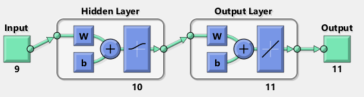
\includegraphics[width=\linewidth]{Figures/Neural Network.png}
    \caption{The implemented neural network model showing the number of input, hidden, and output neurons being utilized.}
\end{figure}

\subsection{Model Summary}
The Input layer has an output shape of (None, 9), representing a flexible batch size and 9 neurons. It doesn't contain any trainable parameters as it simply passes through the input data.

The neural network architecture includes two dense layers. The first dense layer has an output shape of (None, 10), indicating a flexible batch size and 10 neurons. It contains 90 parameters, calculated as $(\text{input\_dim} \times \text{units}) + \text{units} = (8 \times 10) + 10 = 90$, where the input dimension is 9 (8 input features plus 1 bias neuron).

The second dense layer has an output shape of (None, 11), representing 11 neurons in the output layer for the binary output values. It contains 121 parameters, calculated as $(\text{previous\_layer\_units} \times \text{units}) + \text{units} = (10 \times 11) + 11 = 121$, where the previous layer has 10 neurons.

Overall, the total number of parameters in the network is 211, all of which are trainable, with no non-trainable parameters.

\begin{table}[h]
\centering
\normalsize % Increase the font size of the table
\begin{tabular}{|l|l|l|}
\hline
\textbf{Layer (type)} & \textbf{Output Shape} & \textbf{Param \#} \\ \hline
Input & (None, 9) & 0 \\ \hline
Hidden (Dense) & (None, 10) & 90 \\ \hline
Output (Dense) & (None, 11) & 121 \\ \hline
\end{tabular}
\vspace{0.5cm}

\small{
\raggedright{
\hspace{0.8cm}\textbf{Total params:} 211 \\
\hspace{0.8cm}\textbf{Trainable params:} 211 \\
\hspace{-3.5cm}\textbf{Non-trainable params:} 0
}
}
\vspace{0.5cm}
\caption{Neural Network Architecture Summary}
\label{tab:neural_network_architecture}
\end{table}

\subsection{Model Training}
For model development, the dataset was divided into three subsets: 70\% for training (1612 entries), 15\% for validation (345 entries), and 15\% for testing (346 entries). This split ensures that the model is trained on a majority of the data while allowing for evaluation on unseen data to assess generalization performance.

During the training process, we utilized 1000 epochs with a learning rate (Mu) of 0.001. A higher number of epochs allows the model to undergo more iterations, thereby improving its ability to learn complex patterns from the data. Similarly, a lower learning rate helps prevent overshooting of the optimal solution and promotes stable convergence during training. Additionally, we incorporated 100 validation checks to prevent overfitting. This approach ensures that the model achieves optimal convergence and generalization.


\begin{figure}[!htpb]
    \centering
    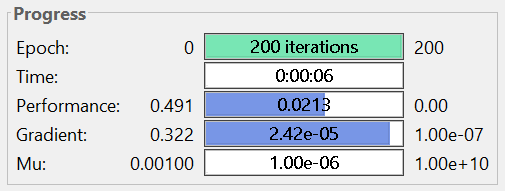
\includegraphics[width=\linewidth]{Figures/testing.png}
    \caption{Training the neural network with these parameters.}
    \label{fig:tcanther}
\end{figure}

During the training process, the neural network employs back propagation to update its weights iteratively. This process involves propagating error backwards through the network and calculating gradients of the loss function with respect to each weight. Specifically using gradient descent, weights are adjusted in small increments to minimize the error. This iterative adjustment continued across multiple epochs until the model converged, as evidenced by the gradient value decreasing to approximately $2.4189 \times 10^{-5}$ by the 200th epoch. At this point, with little to no change in gradients, the training process was stopped as the model had achieved satisfactory performance on the training data.

\begin{figure}[H]
    \centering
    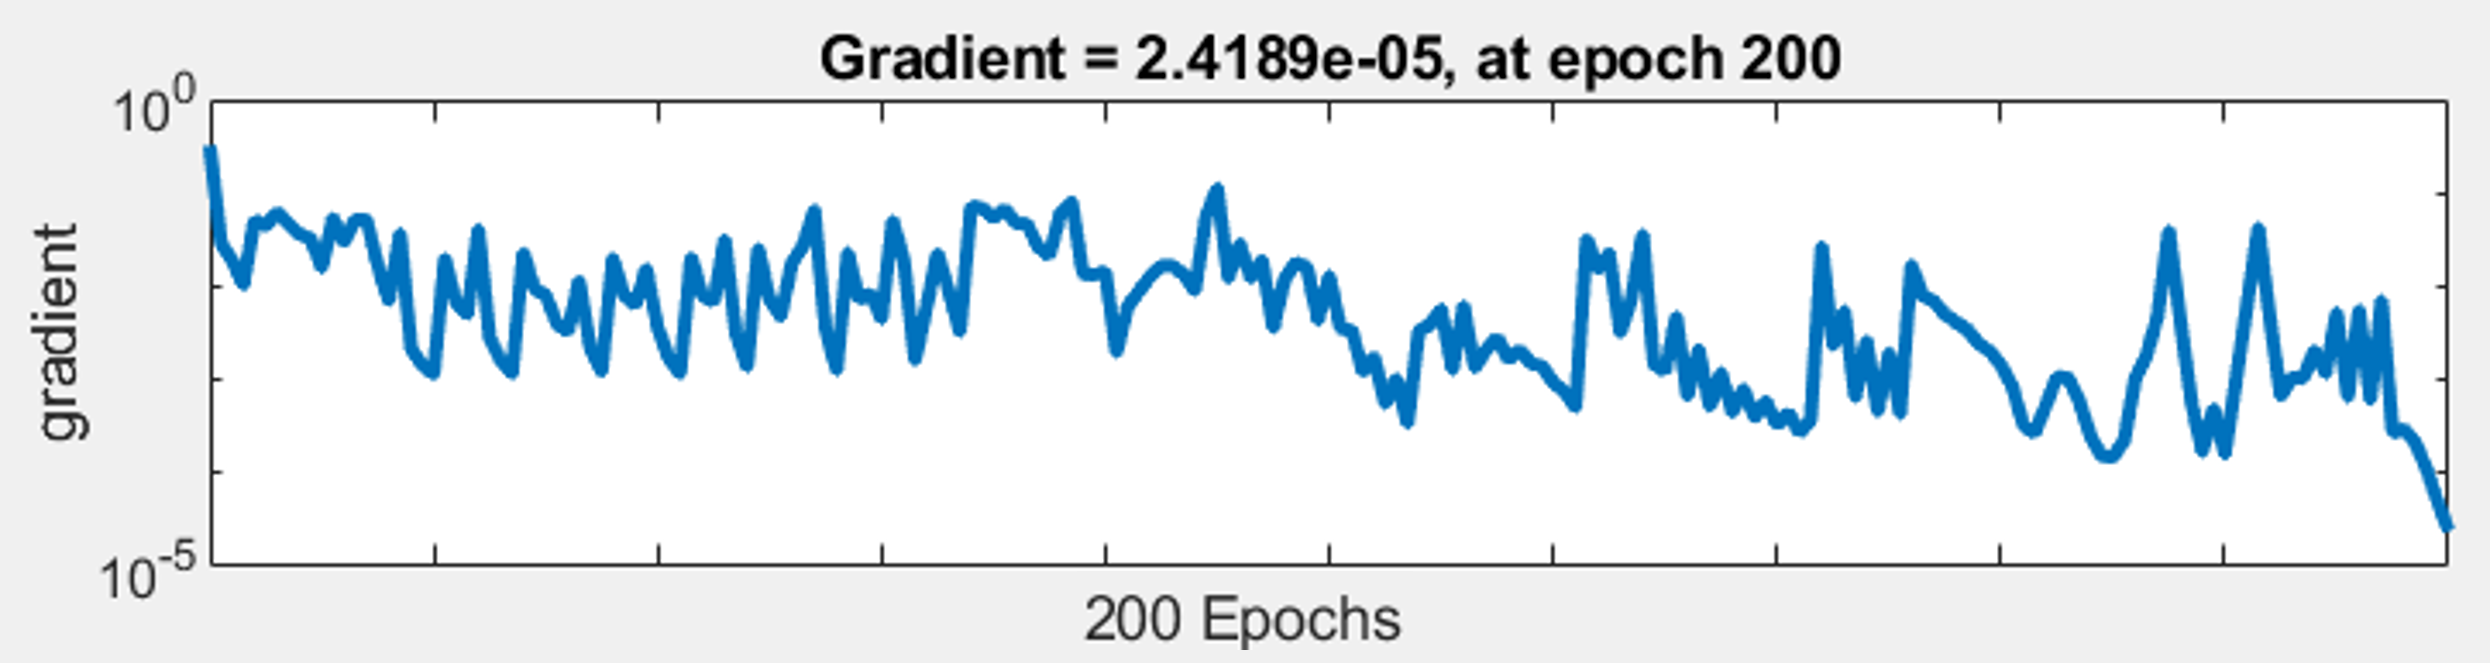
\includegraphics[width=\linewidth]{Figures/gradient2.png}
    \caption{Progression of gradient descent throughout the training iterations of the neural network.}
    \label{fig:tcanther}
\end{figure}

\subsection{Mean Squared Error}
A mean squared error graph was generated, which depicted a decreasing trend, indicating that the model's predictive accuracy improved steadily with each epoch until the curve started approaching towards a horizontal line. The lowest mean squared error achieved was 0.021327, suggesting that the model exhibited optimal performance in minimizing errors between predicted and actual outputs after 200 epochs.

\begin{figure}[!htpb]
    \centering
    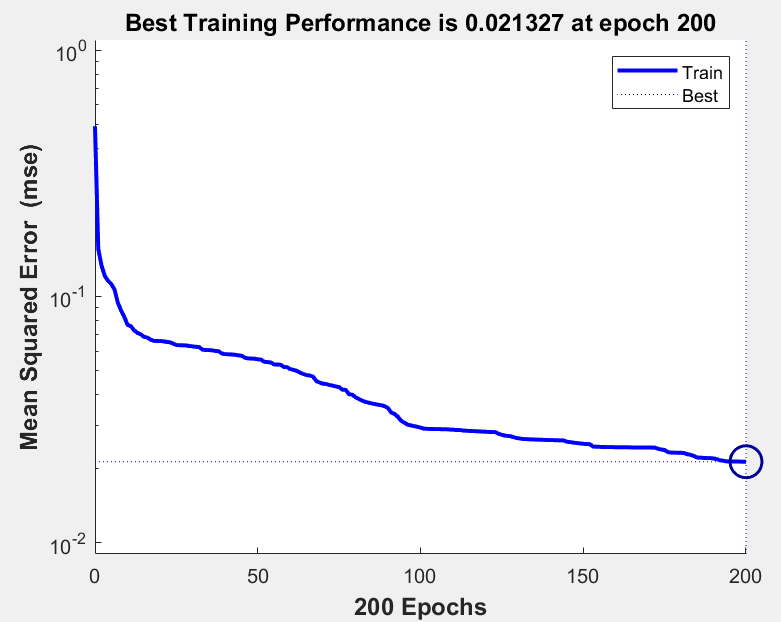
\includegraphics[width=\linewidth]{Figures/MSE2.png}
    \caption{Loss Graph: The decrease in MSE over epochs indicates that the model's predictions gradually converged towards the actual dietary recommendations as training progressed.}
\end{figure}

\subsection{Thresholds}
To ensure that the model's outputs are binary and align with the intended dietary recommendations, thresholds were incorporated into the output layer. These thresholds dictate the point at which the model classifies a recommendation as either present or absent based on the output neurons.